%!TEX root = ../thesis.tex
% ******************************* Thesis Appendix C ********************************

\chapter{Reactor Building Edges} \label{appenC:ReactorBuildingEdges}

\begin{figure}[!h]
 \centering
 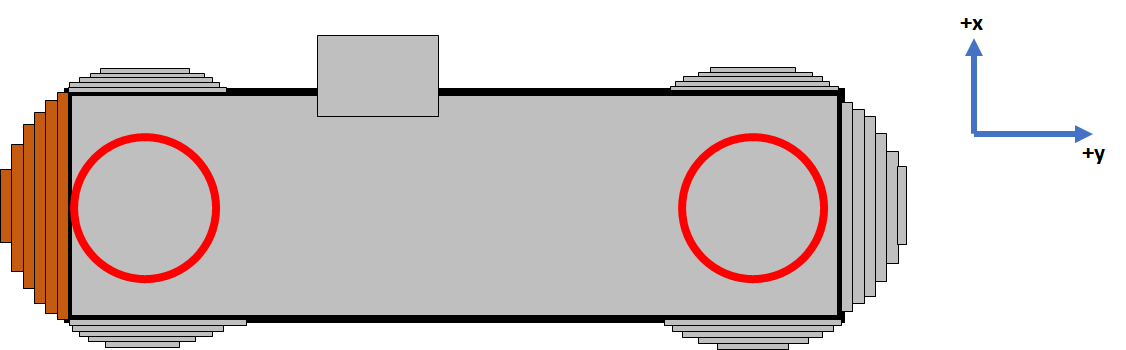
\includegraphics[width=\linewidth]{Chapter5/Figs/wylfaRasterNew/Slabs1.png}
 \captionof{figure}{Slabs for the left middle edge of the reactor building.} 
 \label{fig:slabs1}
\end{figure}

\begin{table*}[!h]
\centering
\begin{tabular}{lrrrrrrr}  
\toprule
\multicolumn{1}{c}{} & \multicolumn{3}{c}{Position} & \multicolumn{3}{c}{Dimension} \\
\cmidrule(r){2-4}
\cmidrule(r){5-7}
Segment       & X\,[m] & Y\,[m] & Z\,[m] & Width\,[m] & Depth\,[m] & Height [m]\\
\midrule
ReactorHSlab1 & 57.5   & -99.8  & 0.0    & 25.0       & 2.0        & 45.0\\
ReactorHSlab2 & 57.5   & -101.8 & 0.0    & 25.0       & 2.0        & 45.0\\
ReactorHSlab3 & 57.5   & -103.8 & 0.0    & 40.1       & 2.0        & 45.0\\
ReactorHSlab4 & 57.5   & -105.8 & 0.0    & 14.3       & 2.0        & 45.0\\
ReactorHSlab5 & 57.5   & -107.8 & 0.0    & 8.4        & 2.0        & 45.0\\
ReactorHSlab6 & 57.5   & -109.8 & 0.0    & 0.0        & 2.0        & 45.0\\
\bottomrule  
\end{tabular}
\caption{Positions and dimensions for figure \ref{fig:slabs1}.}
\label{tab:slabs1}
\end{table*}

\begin{figure}[!h]
 \centering
 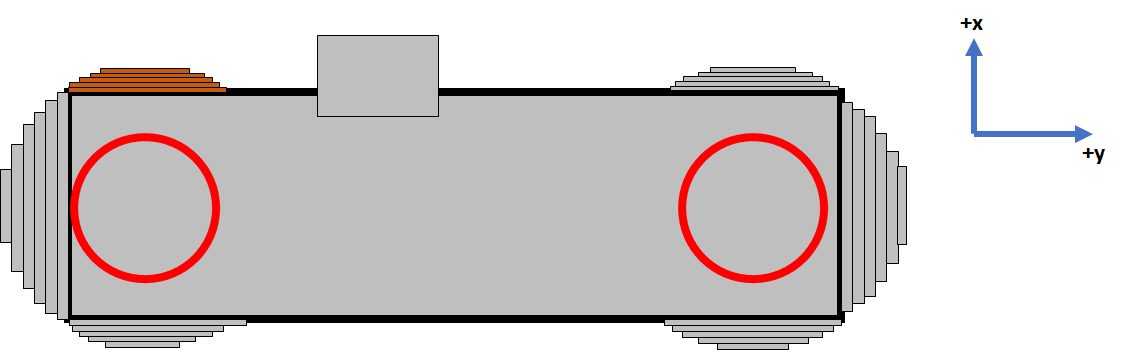
\includegraphics[width=\linewidth]{Chapter5/Figs/wylfaRasterNew/Slabs3.png}
 \captionof{figure}{Slabs for the left upper edge of the reactor building.} 
 \label{fig:slabs3}
\end{figure}

\begin{table*}[!h]
\centering
\begin{tabular}{lrrrrrrr}  
\toprule
\multicolumn{1}{c}{} & \multicolumn{3}{c}{Position} & \multicolumn{3}{c}{Dimension} \\
\cmidrule(r){2-4}
\cmidrule(r){5-7}
Segment       & X\,[m] & Y\,[m] & Z\,[m] & Width\,[m] & Depth\,[m] & Height [m]\\
\midrule
ReactorVSlab1 & 78.2   & -85.3  & 0.0    & 0.9        & 27.9       & 45.0\\
ReactorVSlab2 & 79.1   & -85.3  & 0.0    & 0.9        & 26.3       & 45.0\\
ReactorVSlab3 & 79.9   & -85.3  & 0.0    & 0.9        & 23.4       & 45.0\\
ReactorVSlab4 & 80.8   & -85.3  & 0.0    & 0.9        & 20.1       & 45.0\\
ReactorVSlab5 & 81.7   & -85.3  & 0.0    & 0.9        & 15.7       & 45.0\\
\bottomrule  
\end{tabular}
\caption{Positions and dimensions for figure \ref{fig:slabs3}.}
\label{tab:slabs3}
\end{table*}

\begin{figure}[!h]
 \centering
 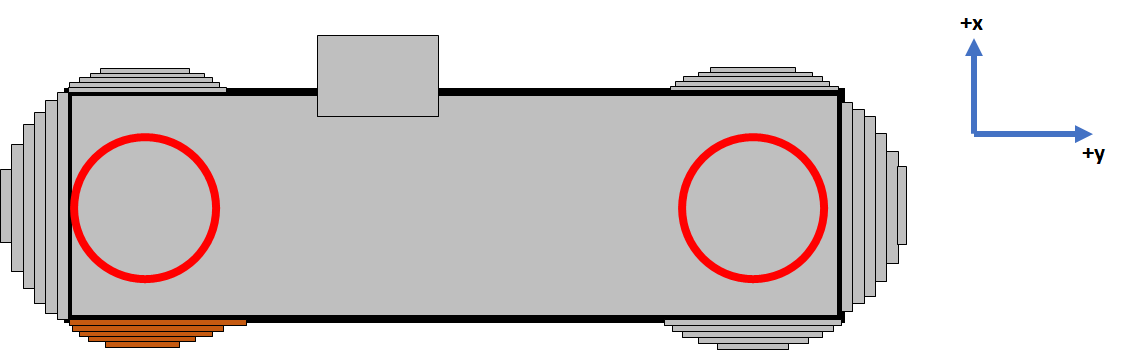
\includegraphics[width=\linewidth]{Chapter5/Figs/wylfaRasterNew/Slabs4.png}
 \captionof{figure}{Slabs for the left lower edge of the reactor building.} 
 \label{fig:slabs4}
\end{figure}

\begin{table*}[!h]
\centering
\begin{tabular}{lrrrrrrr}  
\toprule
\multicolumn{1}{c}{} & \multicolumn{3}{c}{Position} & \multicolumn{3}{c}{Dimension} \\
\cmidrule(r){2-4}
\cmidrule(r){5-7}
Segment        & X\,[m] & Y\,[m] & Z\,[m] & Width\,[m] & Depth\,[m] & Height [m]\\
\midrule
ReactorVSlab6  & 36.8   & -83.2  & 0.0    & 0.9        & 31.3       & 45.0\\
ReactorVSlab7  & 35.9   & -83.2  & 0.0    & 0.9        & 26.7       & 45.0\\
ReactorVSlab8  & 35.1   & -83.2  & 0.0    & 0.9        & 23.5       & 45.0\\
ReactorVSlab9  & 34.2   & -83.2  & 0.0    & 0.9        & 18.9       & 45.0\\
ReactorVSlab10 & 33.3   & -83.2  & 0.0    & 0.9        & 12.9       & 45.0\\
\bottomrule  
\end{tabular}
\caption{Positions and dimensions for figure \ref{fig:slabs4}.}
\label{tab:slabs4}
\end{table*}

\begin{figure}[!h]
 \centering
 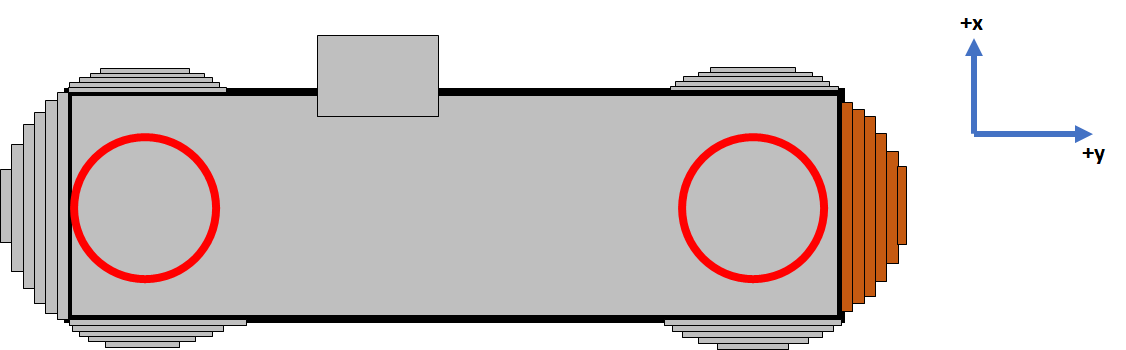
\includegraphics[width=\linewidth]{Chapter5/Figs/wylfaRasterNew/Slabs2.png}
 \captionof{figure}{Slabs for the right middle edge of the reactor building.} 
 \label{fig:slabs2}
\end{figure}

\begin{table*}[!h]
\centering
\begin{tabular}{lrrrrrrr}  
\toprule
\multicolumn{1}{c}{} & \multicolumn{3}{c}{Position} & \multicolumn{3}{c}{Dimension} \\
\cmidrule(r){2-4}
\cmidrule(r){5-7}
Segment        & X\,[m] & Y\,[m] & Z\,[m] & Width\,[m] & Depth\,[m] & Height [m]\\
\midrule
ReactorHSlab7  & 57.5   & 38.2   & 0.0    & 36.9       & 2.0        & 45.0\\
ReactorHSlab8  & 57.5   & 40.2   & 0.0    & 34.2       & 2.0        & 45.0\\
ReactorHSlab9  & 57.5   & 42.2   & 0.0    & 31.7       & 2.0        & 45.0\\
ReactorHSlab10 & 57.5   & 44.2   & 0.0    & 26.1       & 2.0        & 45.0\\
ReactorHSlab11 & 57.5   & 46.2   & 0.0    & 19.7       & 2.0        & 45.0\\
ReactorHSlab12 & 57.5   & 48.2   & 0.0    & 13.7       & 2.0        & 45.0\\
\bottomrule  
\end{tabular}
\caption{Positions and dimensions for figure \ref{fig:slabs2}.}
\label{tab:slabs2}
\end{table*}

\begin{figure}[!h]
 \centering
 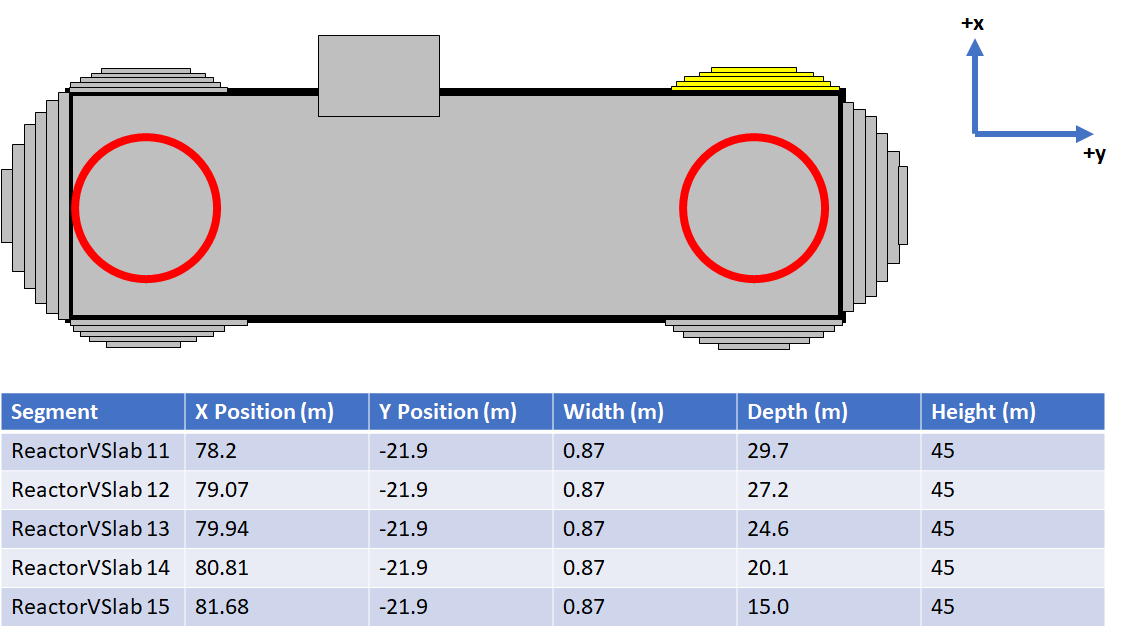
\includegraphics[width=\linewidth]{Chapter5/Figs/wylfaRasterNew/Slabs5.png}
 \captionof{figure}{Slabs for the right upper edge of the reactor building..} 
 \label{fig:slabs5}
\end{figure}

\begin{table*}[!h]
\centering
\begin{tabular}{lrrrrrrr}  
\toprule
\multicolumn{1}{c}{} & \multicolumn{3}{c}{Position} & \multicolumn{3}{c}{Dimension} \\
\cmidrule(r){2-4}
\cmidrule(r){5-7}
Segment        & X\,[m] & Y\,[m] & Z\,[m] & Width\,[m] & Depth\,[m] & Height [m]\\
\midrule
ReactorVSlab11 & 78.2   & -21.9  & 0.0    & 0.9        & 29.7       & 45.0\\
ReactorVSlab12 & 79.1   & -21.9  & 0.0    & 0.9        & 27.2       & 45.0\\
ReactorVSlab13 & 79.9   & -21.9  & 0.0    & 0.9        & 24.6       & 45.0\\
ReactorVSlab14 & 80.8   & -21.9  & 0.0    & 0.9        & 20.1       & 45.0\\
ReactorVSlab15 & 81.7   & -21.9  & 0.0    & 0.9        & 15.0       & 45.0\\
\bottomrule  
\end{tabular}
\caption{Positions and dimensions for figure \ref{fig:slabs5}.}
\label{tab:slabs5}
\end{table*}

\begin{figure}[!h]
 \centering
 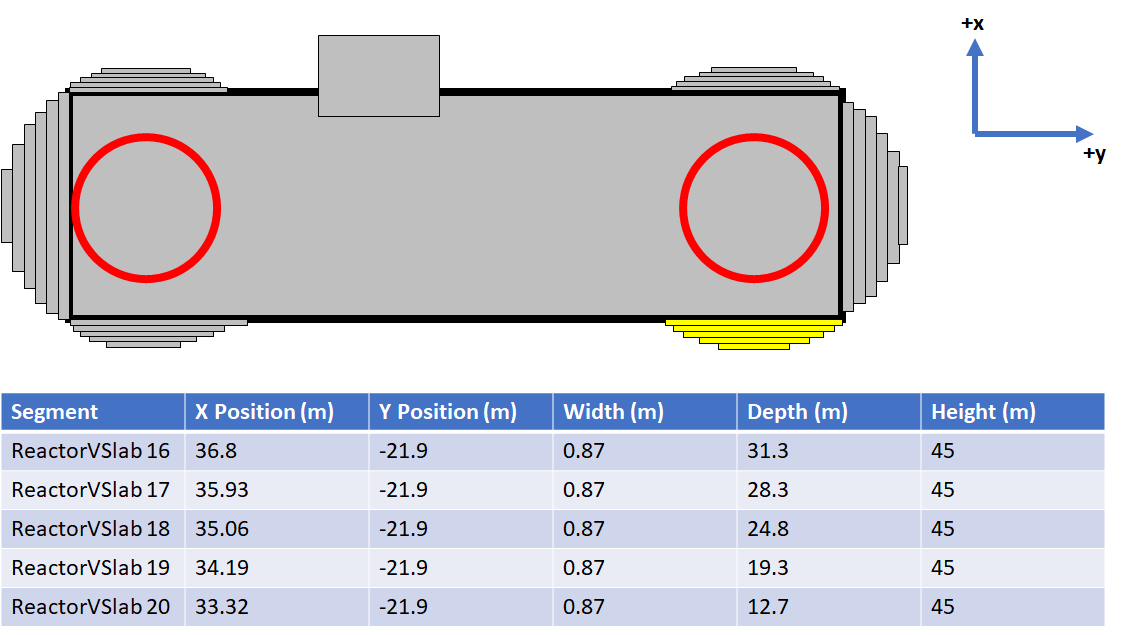
\includegraphics[width=\linewidth]{Chapter5/Figs/wylfaRasterNew/Slabs6.png}
 \captionof{figure}{Slabs for the right lower edge of the reactor building..} 
 \label{fig:slabs6}
\end{figure}

\begin{table*}[!h]
\centering
\begin{tabular}{lrrrrrrr}  
\toprule
\multicolumn{1}{c}{} & \multicolumn{3}{c}{Position} & \multicolumn{3}{c}{Dimension} \\
\cmidrule(r){2-4}
\cmidrule(r){5-7}
Segment        & X\,[m] & Y\,[m] & Z\,[m] & Width\,[m] & Depth\,[m] & Height [m]\\
\midrule
ReactorVSlab16 & 36.8   & -21.9  & 0.0    & 0.9        & 31.3       & 45.0\\
ReactorVSlab17 & 35.9   & -21.9  & 0.0    & 0.9        & 28.3       & 45.0\\
ReactorVSlab18 & 35.1   & -21.9  & 0.0    & 0.9        & 24.8       & 45.0\\
ReactorVSlab19 & 34.2   & -21.9  & 0.0    & 0.9        & 19.3       & 45.0\\
ReactorVSlab20 & 33.3   & -21.9  & 0.0    & 0.9        & 12.7       & 45.0\\
\bottomrule  
\end{tabular}
\caption{Positions and dimensions for figure \ref{fig:slabs6}.}
\label{tab:slabs6}
\end{table*}